%
% $Id: $
%
%
% Compilar a .pdf con LaTeX (pdflatex)
% Es necesario instalar Beamer (paquete latex-beamer en Debian)
%

%
% Gráficos:
% Los gráficos pueden suministrarse en PNG, JPG, TIF, PDF, MPS
% Los EPS deben convertirse a PDF (usar epstopdf)
%

\documentclass[17pt,aspectratio=169]{beamer}
\usetheme[orchid]{Hannover}
%\usebackgroundtemplate{
\includegraphics[width=\paperwidth]{format/libresoft-bg-soft.png}}
\usepackage[spanish]{babel}
\usepackage[utf8]{inputenc}
\usepackage{graphics}
\usepackage{amssymb} % Simbolos matematicos

%\definecolor{libresoftgreen}{RGB}{162,190,43}
%\definecolor{libresoftblue}{RGB}{0,98,143}

%\setbeamercolor{titlelike}{bg=libresoftgreen}

%% Metadatos del PDF.
%% \hypersetup{
%%   pdftitle={La tecnología no es neutra},
%%   pdfauthor={Jesús M. González Barahona},
%%   pdfcreator={GSyC/LibreSoft, Universidad Rey Juan Carlos},
%%   pdfproducer=PDFLaTeX,
%%   pdfsubject={},
%% }
%%

\newcommand\YUGE{\fontsize{48}{60}\selectfont}

\AtBeginSection[]
{
  {
    \usebackgroundtemplate{\includegraphics[width=\paperwidth,height=\paperheight]{\secimage}}
    \begin{frame}<beamer>

      \begin{center}
        {\YUGE\bf\insertsection}
      \end{center}
    \end{frame}
  }
  \renewcommand{\secimage}{figs/bookpages}
}

% Pixbay
% NikolayFrolochkin
% https://pixabay.com/en/book-reading-library-literature-1261800/
% License: CC0 Creative Commons
\newcommand{\secimage}{figs/bookpages}

\begin{document}

\title{¿Qué es el software libre?}
%\subtitle{}
\author{Jesús M. González Barahona}
\institute{Correo: jesus.gonzalez.barahona@urjc.es ~~~~ Fediverso: @jgbarah@floss.social \\
  Universidad Rey Juan Carlos \\ }

\date{Asignatura ``Ética, legislación y profesión'' \\
  Facultad Informática, UCM, 2 de diciembre de 2022\\
{\small \url{https://jgbarah.github.io/presentations}} \\}

\frame{
\maketitle
}
%% \begin{center}
%% 
\includegraphics[width=6cm]{format/gsyc-urjc}
%% \end{center}

%% \begin{frame}

%%   {\Large
%%     \tableofcontents
%%   }

%% \end{frame}

%%---------------------------------------------------------------
%%---------------------------------------------------------------
\section{¿Qué es el software libre?}

%%---------------------------------------------------------------

\begin{frame}

{\small
La mascota de Linux es un pingüino, se llama Tux \\
\url{http://en.wikipedia.org/wiki/Tux} \\
}

\begin{flushright}

\includegraphics[height=5cm]{figs/tux}

{\footnotesize
``Tux'', por Larry Ewing \\
  Vía Wikimedia Commons \url{http://commons.wikimedia.org/wiki/File:Tux.png}
}
\end{flushright}

\end{frame}

%%---------------------------------------------------------------

\begin{frame}

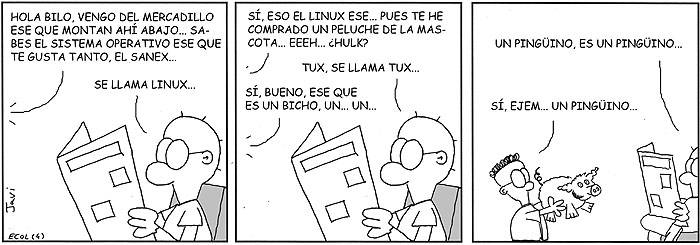
\includegraphics[height=4cm]{figs/tiraecol-5}

\begin{flushright}
``Linux, ese gran desconocido'' \\
{\small TiraEcol, \url{https://github.com/nasciiboy/tira-ecol}}
\end{flushright}

\vspace{.5cm}

\begin{center}
{\huge
El software libre, ese gran desconocido
}
\end{center}

\end{frame}

%%---------------------------------------------------------------

\begin{frame}
\frametitle{Ese desconocido}

\begin{center}
  {\Large
  El software libre \\
  es omnipresente en la industria \\
  pero \\
  muy pocos lo entienden \\
  o incluso le prestan atención \\
  }
\end{center}

\end{frame}

%%---------------------------------------------------------------

\begin{frame}
\frametitle{¿Qué es el software libre?}

El autor otorga permiso:

\begin{itemize}
\item uso, sin limitaciones
\item estudio y modificación
\item redistribución
\item redistribución de versiones modificadas
\end{itemize}

Imprescindible: disponibilidad de código fuente

\end{frame}

%%---------------------------------------------------------------

\begin{frame}
\frametitle{¿Y por qué es esto y no otra cosa?}

\begin{itemize}
\item Motivos éticos: \\
  {\em ``porque las cosas deberían ser así''} \\
\item Motivos prácticos: \\
  {\em ``porque las cosas funcionan mejor así''} \\
\end{itemize}

\end{frame}

%%---------------------------------------------------------------

\begin{frame}
\frametitle{Definiciones de consenso}

\begin{itemize}
\item Definición de la Free Software Foundation
\item Debian Free Software Guidelines, 
\item Definición de ``Open Source''.
\end{itemize}

\begin{flushright}
{\footnotesize
  \url{https://www.gnu.org/philosophy/free-sw.en.html} \\
  \url{https://www.debian.org/social_contract\#guidelines} \\ 
  \url{https://opensource.org/osd} \\
}
\end{flushright}

\end{frame}

%%---------------------------------------------------------------
%%---------------------------------------------------------------
\section{Consecuencias, características}

%%---------------------------------------------------------------

\begin{frame}
\frametitle{Consecuencias}

{\small
  \begin{itemize}
\item \textbf{Sostenibilidad}: modelo radicalmente distinto
\item \textbf{Apertura}: puede modificarse, inspeccionarse,
  estudiarse
\item \textbf{Distribución}: nuevos canales, nuevos métodos
\item \textbf{Desarrollo}: modelos de desarrollo ``sorprendentes''
\item \textbf{Mantenimiento y soporte}: Verdadera competencia
\item \textbf{Seguridad}: No más seguridad por ocultación
\end{itemize}
}
\end{frame}


%%---------------------------------------------------------------

\begin{frame}
\frametitle{Combinación de dos poderosos mecanismos}

{\Large
  \begin{itemize}
  \item Competencia \\
    (usando todos la misma base)
  \item Cooperación \\
    (incluso involuntaria)
\end{itemize}
}
\end{frame}

%%---------------------------------------------------------------

\begin{frame}
\frametitle{La importancia de la transparencia}

{\small
No sólo el código es importante:

\begin{itemize}
\item también el proceso de desarrollo...
\item ...la comunidad alrededor del proyecto...
\item ...y el ecosistema de proyectos que le rodea
\end{itemize}

Para tomar decisiones a medio y largo, \\
hay que tenerlo en cuenta \\
}
\end{frame}

%%---------------------------------------------------------------

\begin{frame}
\frametitle{Calidad}

{\small

Mecanismos novedosos para conseguir calidad

\begin{itemize}
\item Mejora incremental
\item Pruebas realizadas por la comunidad
\item Revisión por pares \\
  (pre-commit, post-commit, over the lifetime) \\
\item Transparencia (incluyendo errores)
\item Efecto ``vergüenza torera''
\item Auditoría por terceros
\item ...y en muchos casos, mecanismos tradicionales
\end{itemize}

}
\end{frame}

%%---------------------------------------------------------------

\begin{frame}
\frametitle{Calidad}

\begin{center}
  {\bf Todos los atributos de calidad \\
    pueden evaluarse \\
    sin compromiso con el productor \\}
\end{center}
\end{frame}

%%---------------------------------------------------------------

\begin{frame}
\frametitle{Seguridad}

\begin{itemize}
\item No hay seguridad por ocultación
\item Efecto ``muchos ojos'' (escrutinio público)
\item Incentivos para reportar problemas
\item Incentivos para corregir problemas
\item Auditorías completas de seguridad posibles
\item Mecanismos tradicionales
\end{itemize}

\end{frame}

%%---------------------------------------------------------------

\begin{frame}
\frametitle{Seguridad}

Aún así, puede haber problemas:

\begin{itemize}
\item Ejemplos: ¿hace falta darlos?
\item En general, poco tiempo detección - corrección
\item Ojo: hay que desplegar la actualización
\end{itemize}
\end{frame}

%%---------------------------------------------------------------

\begin{frame}
\frametitle{Innovación incremental}

\begin{itemize}
\item Aportaciones incrementales a un producto base
\item Ciclos de innovación y realimentación rápidos
\item Mejora y despliegue continuo
\item Habitualmente, dirigido por usuarios
\item Modelo en comunidades de software libre \\
  (Linux, Apache, OpenStack, ...) \\
\end{itemize}

\end{frame}

%%---------------------------------------------------------------

\begin{frame}
\frametitle{Mejora disruptiva}

\begin{itemize}
\item Pequeña pieza de software marca la diferencia
\item Todo el resto: software libre
\item Modelo en Silicon Valley \\
  (Google, Meta, Amazon, muchísimas startups) \\
\end{itemize}

\end{frame}

%%---------------------------------------------------------------
%%---------------------------------------------------------------
\section{Licencias}

%%---------------------------------------------------------------

\begin{frame}
\frametitle{Fundamento legal}

\begin{itemize}
\item Legislación sobre copyright:
  no se puede hacer casi nada con un programa
  que se recibe o se compra
\item Licencias de software libre: garantizan permisos
\item Si redistribuyes un programa, has de hacerlo cumpliendo su licencia
\end{itemize}

\end{frame}

%%---------------------------------------------------------------

\begin{frame}
\frametitle{Quién determina la licencia}

\begin{itemize}
\item Obra individual: su autor \\
  o a quien ceda derechos
\item Obra colectiva: sus autores \\
  o a quien cedan derechos
\end{itemize}

\end{frame}

%%---------------------------------------------------------------

\begin{frame}
\frametitle{Escenarios comunes}

\begin{itemize}
\item Derechos de una empresa(s): \\
  software producido por sus empleados
\item Cesión a una fundación: \\
  defensa en nombre de autores
\item Derechos de los contribuidores: \\
  hay respetarlos para contribuciones ``significativas''
\item ``Licencia implícita'': \\
  contribuciones afectadas por la licencia
\end{itemize}

\end{frame}

%%---------------------------------------------------------------
%%---------------------------------------------------------------
\section{Ejemplos de licencias}

%%---------------------------------------------------------------

\begin{frame}
\frametitle{BSD (Berkeley Software Distribution)}

\begin{itemize}
\item Versiones de Unix BSD.
\item Obliga a dar crédito a los autores.
\item Permite redistribución binaria.
\item Permite (pero no obliga) redistribución fuente
\item Permite modificaciones e integración
\item Licencias similares: MIT, Artistic (Perl)
\end{itemize}

\begin{flushright}
  {\small
    \url{https://en.wikipedia.org/wiki/BSD_licenses}
  }
\end{flushright}
\end{frame}

%%---------------------------------------------------------------

\begin{frame}
\frametitle{GPL (GNU Public License)}

\begin{itemize}
\item Software de FSF (y mucho más, como Linux)
\item Ingeniería legal (copyleft).
\item Permite redistribución binaria.
\item Permite redistribución fuente \\
  (obliga en caso de redistribución binaria).
\item Permite modificaciones sin restricciones.
\item Integración completa sólo con software GPL.
\end{itemize}

\begin{flushright}
  {\small
    \url{https://www.gnu.org/licenses/gpl-3.0.en.html}
  }
\end{flushright}

\end{frame}

%%---------------------------------------------------------------

\begin{frame}
\frametitle{LGPL (Lesser GPL)}

\begin{itemize}
\item Bibliotecas de FSF (y mucho más).
\item Pensada para permitir el uso de bibliotecas libres con software
  propietario..
\item Como GPL si se redistribuye la biblioteca como tal.
\item Permite integración con otro software.
\end{itemize}

\begin{flushright}
  {\small
    \url{https://www.gnu.org/licenses/lgpl-3.0.en.html}
  }
\end{flushright}

\end{frame}

%%---------------------------------------------------------------

\begin{frame}
\frametitle{Otras licencias}

\begin{itemize}
\item Affero GPL: \\
  no se puede desactivar descarga de código fuente.
\item Eclipse Public License: \\
  copyleft ``ligero''
\item European Union Public License: \\
  copyleft, traducida a idiomas de la UE
\end{itemize}

\end{frame}

%%---------------------------------------------------------------

\begin{frame}
\frametitle{Licenciamiento dual}

\begin{itemize}
\item El autor puede distribuir con varias licencias
\item En algunos casos, el código es exactamente igual
\item Estrategia empleada por algunas empresas \\
  (modelo MySQL)
\item Open core: parte es privativa \\
  no es realmente licenciamiento dual
\end{itemize}

\end{frame}

%%---------------------------------------------------------------

\begin{frame}
\frametitle{Para terminar}

\begin{itemize}
\item GPL: maximiza la libertad \\
  de quien recibe el programa
\item BSD: maximiza la libertad \\
  de quien redistribuye
\item Importante: decidir la licencia pronto
\item La licencia impacta \\
  en el modelo de sostenibilidad
\end{itemize}

\end{frame}

%%---------------------------------------------------------------
%%---------------------------------------------------------------
\section{¿Es la licencia suficiente?}

%%---------------------------------------------------------------

\begin{frame}
\frametitle{Desarrollo abierto}

¿Cómo es el proceso de desarrollo?

\begin{itemize}
\item ¿Hay información sobre todos los cambios?
\item ¿Se conocen los procesos de desarrollo?
\item ¿Pueden consultarse los sistemas de apoyo al desarrollo?
\item ¿Pueden analizarse sus datos?
\item ¿Se conocen los planes a futuro?
\item ¿Cómo es la toma de decisiones?
\end{itemize}

\end{frame}

%%---------------------------------------------------------------

\begin{frame}
\frametitle{Equipo abierto}

¿Cómo es el equipo de desarrollo?

\begin{itemize}
\item ¿Cómo se entra en el equipo de desarrollo?
\item ¿Cómo se reparten las responsabilidades?
\item ¿Quién lo financia?
\item ¿Qué metas tiene? (y ¿quién las fija?)
\item ¿Cómo se relaciona con la comunidad?
\end{itemize}

\end{frame}


%%---------------------------------------------------------------

\begin{frame}
\frametitle{Comunidad abierta}

¿Cómo es la comunidad alrededor del proyecto?

\begin{itemize}
\item ¿Hay canales de comunicación fluidos y públicos?
\item ¿Qué influencia tiene sobre el desarrollo?
\item ¿Quién pone los recursos para que funcione?
\item ¿Está organizada?
\item ¿Qué mecanismos de decisión tiene?
\item ¿Quién participa en ella?
\end{itemize}

\end{frame}

%%---------------------------------------------------------------
\begin{frame}

  \begin{center}
    {\Huge Más allá\\ del código fuente\\ y su licencia...\\}
  \end{center}

\end{frame}

%%---------------------------------------------------------------
%%---------------------------------------------------------------
\section{Software libre como infraestructura}


%%---------------------------------------------------------------
\begin{frame}

  \begin{center}
    {\Large ¿Un nuevo modelo\\
      para la interdepencia\\
      (y la independencia)\\
      tecnológica?\\}
  \end{center}

\end{frame}


%%---------------------------------------------------------------
%%---------------------------------------------------------------
\section{Investigación abierta}

%%---------------------------------------------------------------
\begin{frame}

  \begin{center}
    {\Large \em''Que el conocimiento\\
      generado por la investigación\\
      esté accesible para la sociedad''\\}
  \end{center}

  \begin{itemize}
  \item publicaciones
  \item datos
  \item muestras
  \item software
  \item ...
  \end{itemize}

\end{frame}

%%---------------------------------------------------------------
\begin{frame}

  \begin{center}
    {\Large ¿No es esto lo que siempre ha perseguido la ciencia?\\}
  \end{center}

  \vspace{1cm}
  
  \begin{flushright}
    {\em ``Si he visto más lejos\\
    es porque estoy sentado\\
    sobre los hombros de gigantes''\\}
  \vspace{.3cm}
    {\small (Isaac Newton, carta a Robert Hooke, 1676)\\}
  \end{flushright}
\end{frame}

%%---------------------------------------------------------------

\begin{frame}
\frametitle{Prácticas de investigación abierta}

\begin{itemize}
\item Publicación en acceso abierto (\emph{open access})
\item Datos abiertos (\emph{open data})
\item Software libre
\item Hardware libre
\item Recursos educativos abiertos
\item Evaluación y revisión abierta
\end{itemize}

\end{frame}

%% ---------------------------------------------------------------

\begin{frame}
\frametitle{El software libre como modelo}

\begin{itemize}
\item Apertura de todo el proceso de investigación
\item Uso intensivo de publicación digital abierta
\item Herramientas telemáticas de colaboración
\item Proceso continuo, y no sólo tras la publicación
\item Colaboración: ciencia hecha en comunidades
\end{itemize}

\end{frame}

%% ---------------------------------------------------------------

\begin{frame}
\frametitle{Nuevas posibilidades}

\begin{itemize}
\item Colaboración en grupos enormes
\item Colaboración de profesionales y aficionados
\item Ciencia ciudadana
\item Compromiso de agentes interesados
\item Líneas de investigación y desarrollo interrelacionadas
\end{itemize}

\begin{center}
  {\Large \em Comunidades de investigación}
\end{center}
\end{frame}

%%---------------------------------------------------------------
%%---------------------------------------------------------------
\section{Acabamos...}

%%---------------------------------------------------------------

\begin{frame}

  \begin{center}
  {\Large
    El software libre tiene ya \\
    unos 35 años\\

    \vspace{.5cm}
    
    Ha mostrado el camino\\
    en muchos ámbitos\\

    \vspace{.5cm}
    
    ¿Tiene que renovarse y redefinirse?\\
    ¿Puede ser estrategia de futuro?\\
  }
  \end{center}
\end{frame}

%%---------------------------------------------------------------
% LICENCIA DE REDISTRIBUCION DE LAS TRANSPAS
\frame{
~
\vspace{3cm}

\begin{flushright}
{\small
\copyright 2000-2022 Jesús M. González Barahona. \\

  Algunos derechos reservados. \\
  Este artículo se distribuye bajo la licencia \\
  ``Reconocimiento-CompartirIgual 4.0 Internacional'' \\
  de Creative Commons, \\
  disponible en \\
}
{\footnotesize
  \url{https://creativecommons.org/licenses/by-sa/4.0/} \\
}
\end{flushright}
}

\end{document}

%%% Local Variables:
%%% mode: latex
%%% TeX-master: t
%%% End:
